\documentclass{beamer}

\usepackage[utf8]{inputenc}
\usepackage{default}
\usepackage{graphicx}

\usetheme[secheader]{Madrid}
\useoutertheme{infolines}
\title{Qt-Designer}
\author{Barthez Vinent - Fiore Cyrille}

\begin{document}

\section{Qt-Designer}
\begin {frame}{Qt-Designer}
\maketitle
\end{frame}

\begin {frame}[fragile]{Sommaire}
 \begin{enumerate}
  \item Qu'est ce que Qt-designer ?
  \item A quoi sert Qt-designer ?
  \item Le fonctionnement.
  \item L'intégration dans Qt Creator.
 \end{enumerate}
\end{frame}

\section{Qu'est ce que Qt-designer ?}
\begin{frame}[fragile]{Qu'est ce que Qt-Designer ?}
 \begin{itemize} [<+-|alert@+>]
  \item Outil de developpement.
  \item Complément de Qt-Creator: fait parti du Qt Frameworks
  \item ``Concepteur d'interface''
 \end{itemize}
\end{frame}

\begin{frame}[fragile]{Un peu d'histoire}
Qt est une bibliothèque multi-plateforme développée en C++, créée en 1994.
\pause
 \begin{itemize} [<+-|alert@+>]
  \item 1995: Qt1 - Première version de Qt ouverte au public
  \item 2005: Qt4 - Première version de Qt séparée en modules \\
  Apparition de Qt Designer
 \end{itemize}
\end{frame}

\section{A quoi sert Qt-designer ?}
\begin{frame}[fragile]{A quoi sert Qt-designer ?}
C'est un outil de création d'interface graphique.
\pause
 \begin{itemize} [<+-|alert@+>]
  \item Creations de fenêtres et widgets
  \item Gestion basique des signaux
  \item Genère des fichiers .ui
 \end{itemize}
\end{frame}

\begin{frame}[fragile]{L'interface}
 \begin{center}
  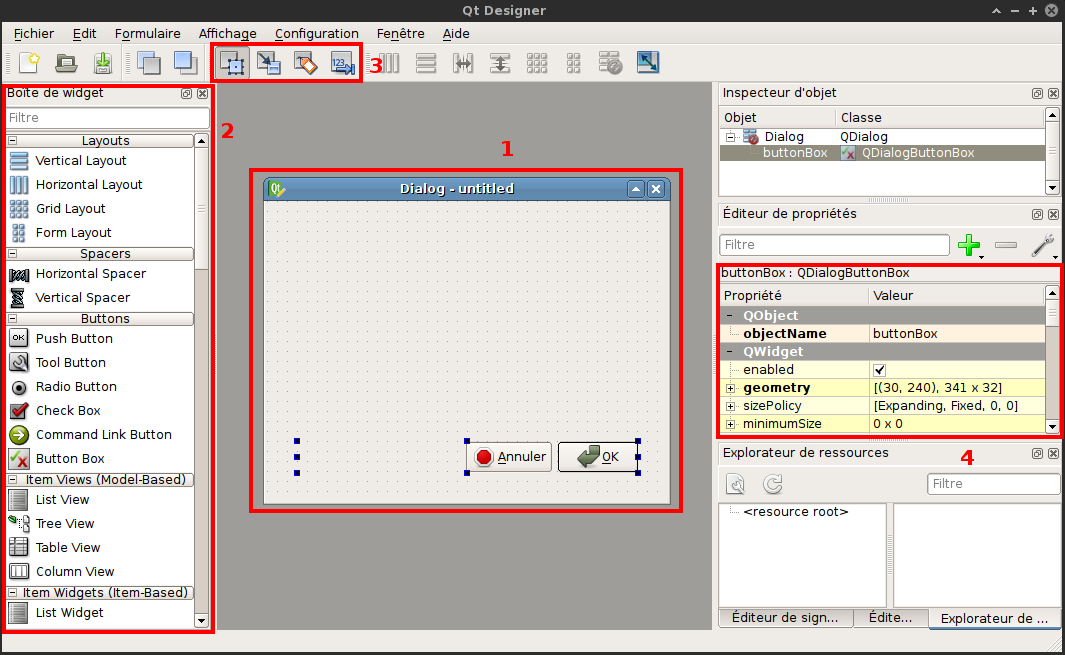
\includegraphics[scale=0.30]{InterfaceGenerale.png}
 \end{center}
\end{frame}

\begin{frame}[fragile]{Les buttons}
 \begin{center}
  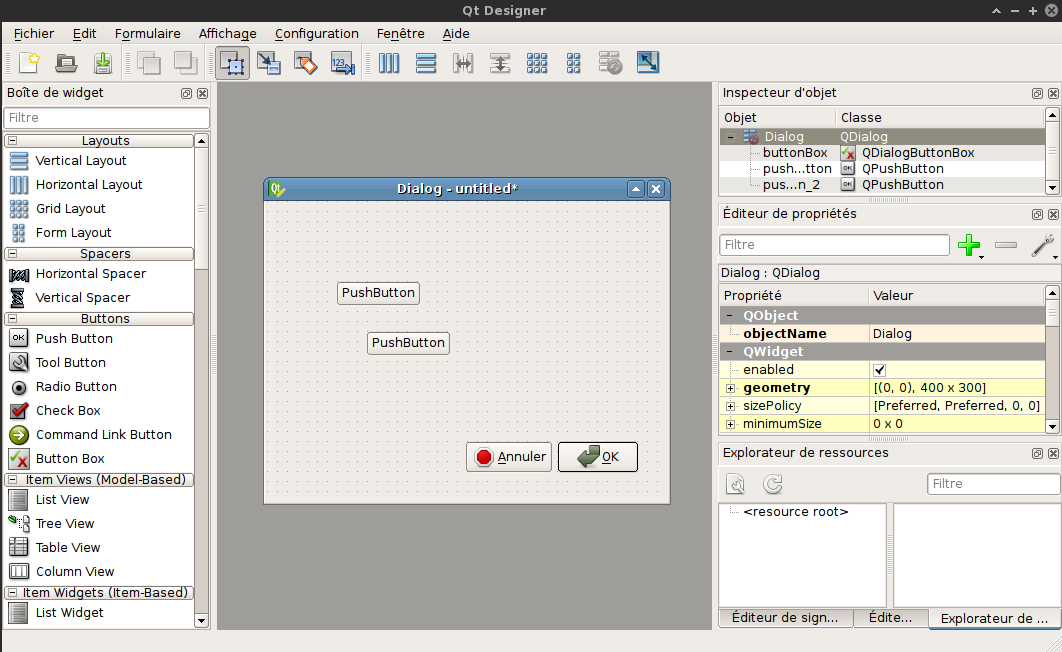
\includegraphics[scale=0.30]{Sanslayout.png}
 \end{center}
\end{frame}

\begin{frame}[fragile]{Les layouts}
 \begin{center}
  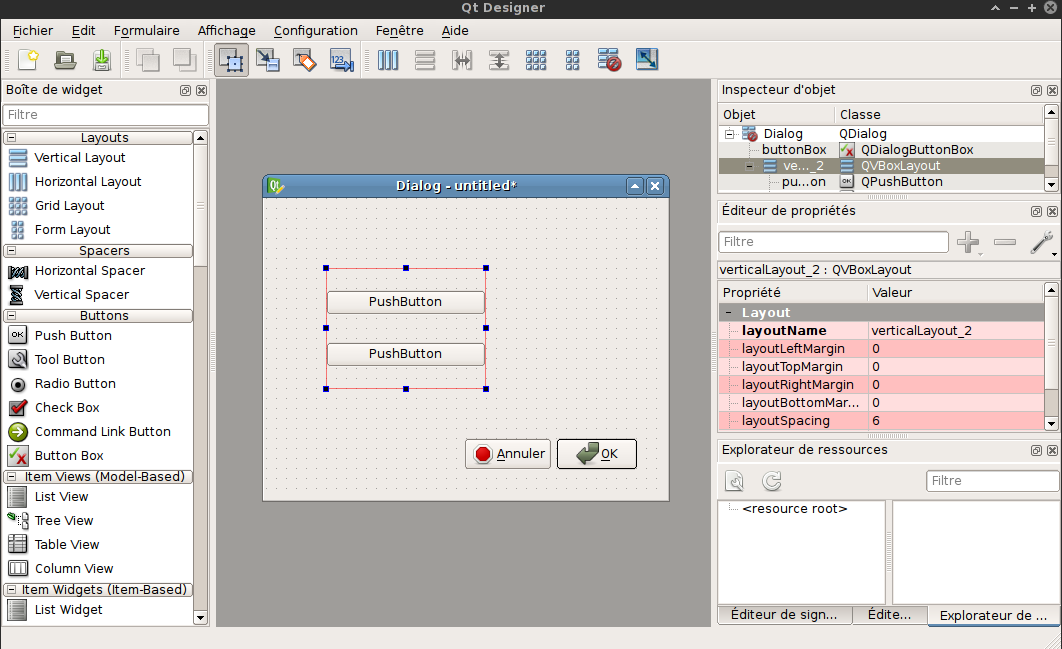
\includegraphics[scale=0.30]{Layout.png}
 \end{center}
\end{frame}

\begin{frame}[fragile]{Les spacers}
 \begin{center}
  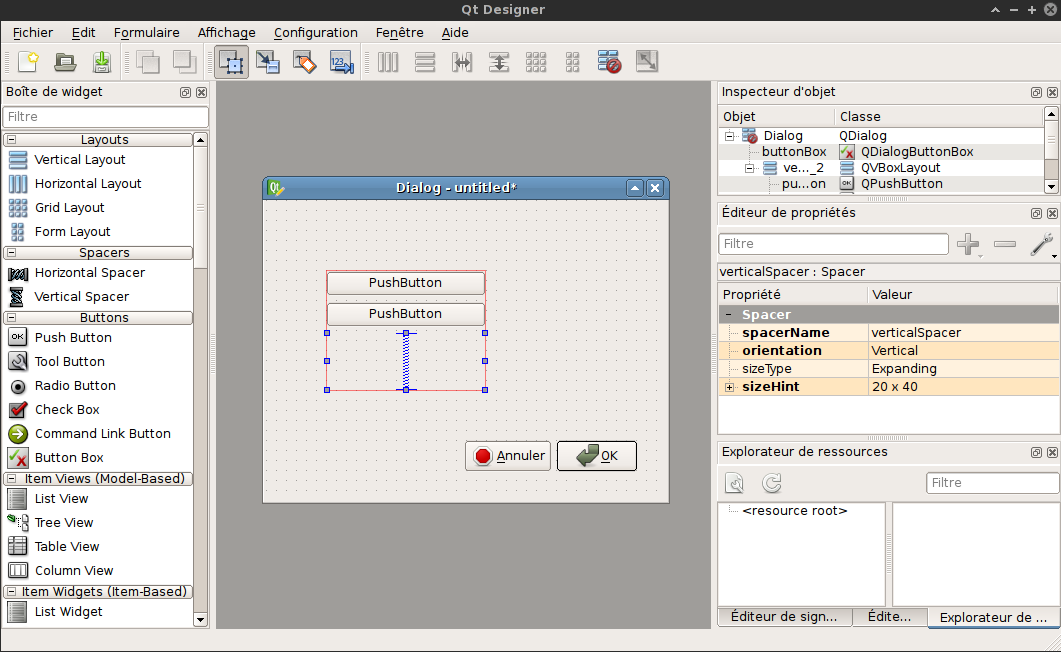
\includegraphics[scale=0.30]{Layoutavecspacer.png}
 \end{center}
\end{frame}

\begin{frame}[fragile]{L'éditeur de signaux}
 \begin{center}
  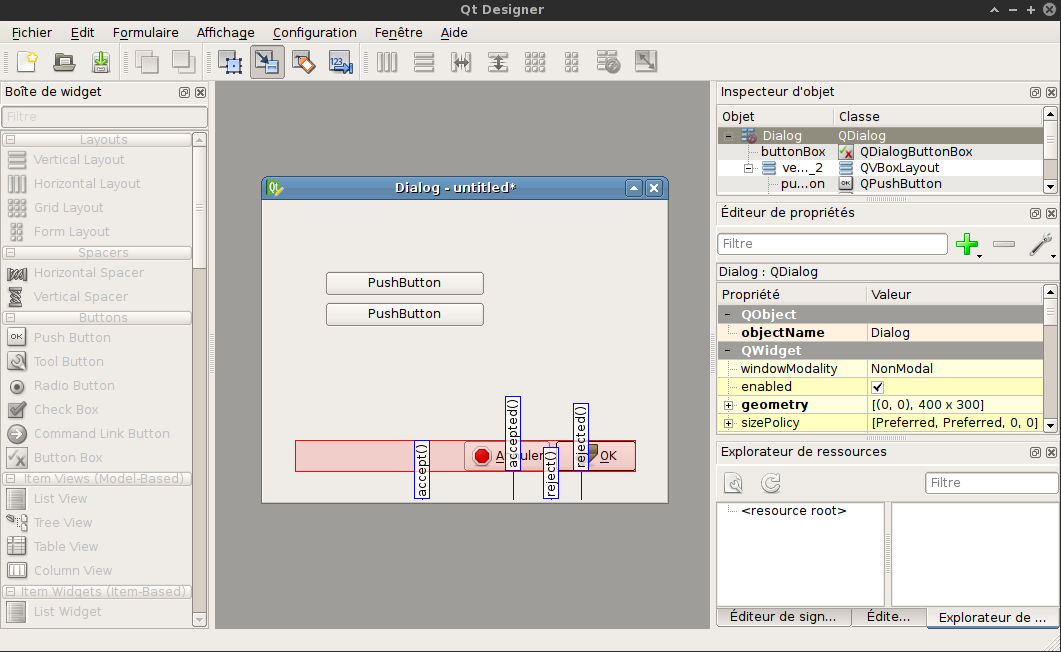
\includegraphics[scale=0.30]{Signaux1.png}
 \end{center}
\end{frame}

\begin{frame}[fragile]{L'éditeur de signaux}
 \begin{center}
  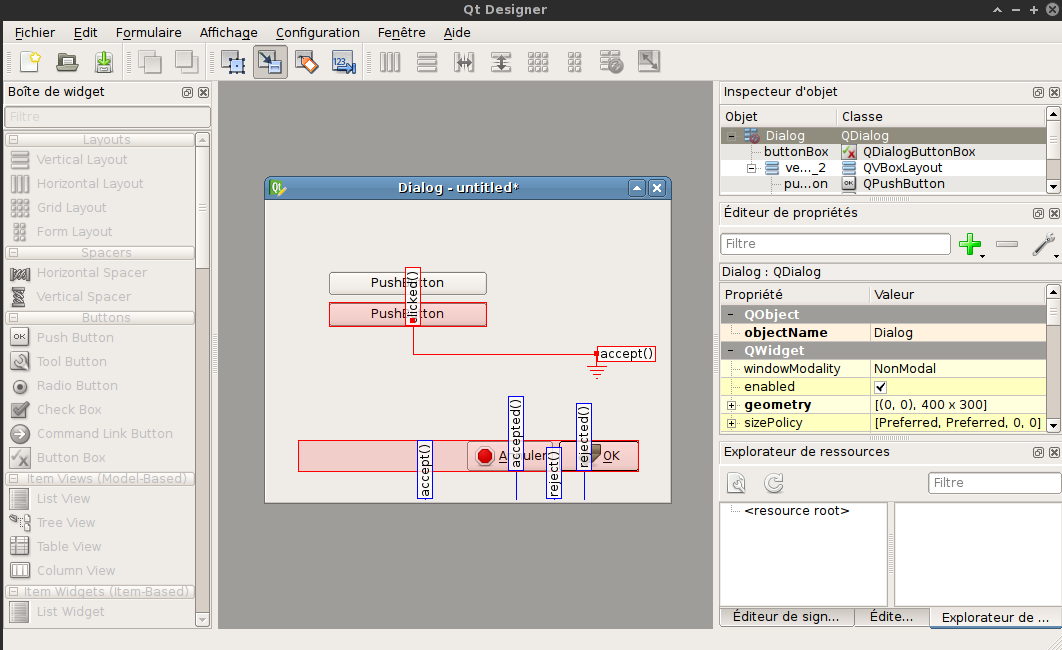
\includegraphics[scale=0.30]{Signaux2.png}
 \end{center}
\end{frame}

\begin{frame}[fragile]{L'éditeur de signaux}
 \begin{center}
  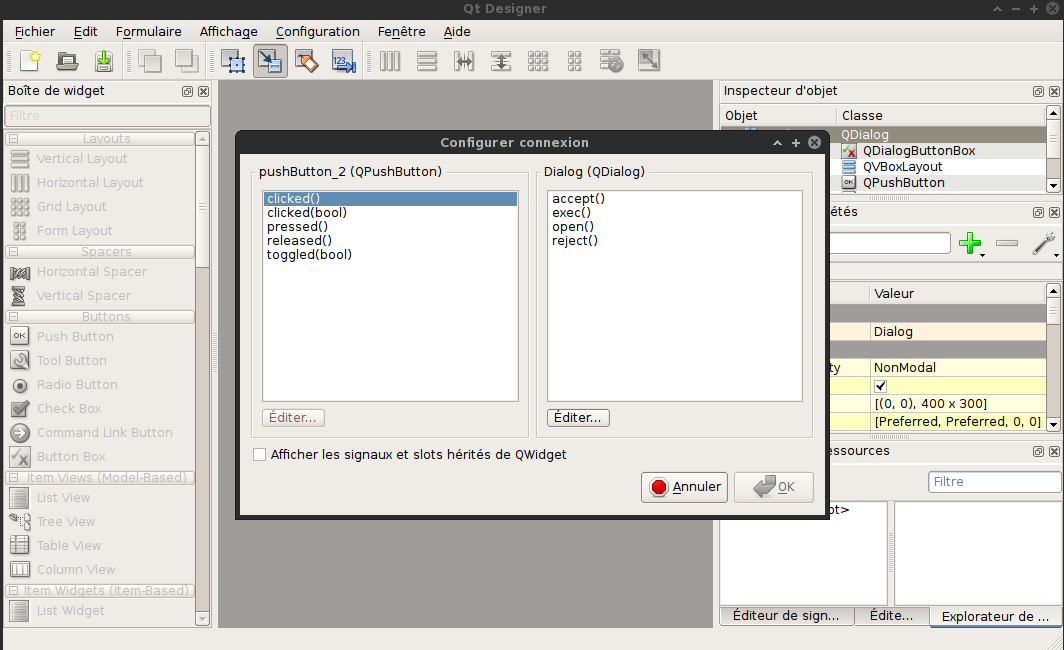
\includegraphics[scale=0.30]{Signaux3.png}
 \end{center}
\end{frame}

\section{Le fonctionnement}
\begin{frame}[fragile]{Les fichiers .ui}
 \begin{enumerate}
  \item Qt Designer génère des fichiers .ui
  \item uic transforme les fichiers .ui en .h
  \begin{center}
   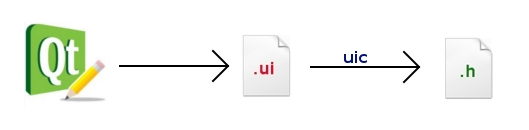
\includegraphics[scale=0.60]{comp.jpg}
  \end{center}
 \end{enumerate}
\end{frame} 

\begin {frame}[fragile]{Les fichiers .ui}
 \begin{enumerate}
  \item widget
  \item property
  \item layout
  \item connection
 \end{enumerate}
\end{frame}

\begin {frame}[fragile]{La balise connection}
 \begin{enumerate}
  \item sender
  \item signal
  \item reciever
  \item slot
 \end{enumerate}
\end{frame}

\begin {frame}[fragile]{Le .h}
 \begin{itemize} [<+-|alert@+>]
  \item Inclusion des headers nécéssaires de Qt
  \item Déclaration des widgets de la fenêtre (attributs)
  \item Une méthode setupUi()
  \item Une méthode retranslateUi()
 \end{itemize}
\end{frame}

\section{L'intégration dans Qt Creator}
 \begin {frame}{Compilation} 
Le .h correspondant au .ui n'est pas éditable par défault dans Qt Creator, en effet, celui ci est généré au moment de la compilation (et donc toute modification est écrasée).\newline \newline

Dans le Makefile, on a :\newline \newline

ui\_mainwindow.h: mainwindow.ui\newline
/usr/bin/uic mainwindow.ui -o ui\_mainwindow.h
\end {frame}

\begin {frame}[fragile]{Signaux/Slots personalisés}
 \begin{itemize} [<+-|alert@+>]
  \item Il faut écrire son propre code.
  \item Les slots personalisés sont à déclarer dans un header.
  \item Qt Designer peut tout de même générer les entêtes et les déclarations.
 \end{itemize}
\end{frame}

\section{Sources}
\begin {frame}[fragile]{Sources}
 \begin{enumerate}
  \item http://www.wikipedia.org/
  \item http://stackoverflow.com/
  \item http://www.siteduzero.com/
 \end{enumerate}
\end{frame}

\end{document}
